After we have shown a set of possible solutions with the frequency controllers,we provide a now an approach in the state-space domain. This is possible thanks to the estimation made through the \textit{greyest} function by Matlab.\\
Before applying the pole placement, we have built a full-state observer and checked that all the states are properly estimated as shwon previously. As consequence, we tuned the pole placement taking the estimated states coming out from the above-mentioned observer. 
\section{1-DOF}
The estimated states are so $\hat{\theta_{l}}$, $\hat{\dot{\theta_{l}}}$, $\hat{\theta_{1}}$,  $\hat{\dot{\theta_{1}}}$. 
We will use the following block scheme:
%FIGURA
A pole placement directly applied to the system is not sufficient to reach the reference, to overcome this problem we decided to apply an integrator. To do so, we need to enlarge the system adding a state $v(t)$; the resulting enlarged state space system is the following one:

\begin{equation}
	\begin{bmatrix}
		\dot{\theta_l} \\
		\ddot{\theta_l} \\
		\dot{\theta_1} \\
		\ddot{\theta_1} \\
		\dot{v}
	\end{bmatrix}
	=
	\begin{bmatrix}
		0 &1 & 0 & 0 & 0 \\
		-\frac{K_{s_1}}{J_m} & -\frac{B_m}{J_m}-\frac{\eta_m \eta_g k_t k_m {K_g}^2}{R_m J_m}  & \frac{K_{s_1}}{J_m} & 0 & 0 \\
		0 & 0 & 0 & 1 & 0 \\
		\frac{K_{s_1}}{J_1} & 0 & -\frac{K_{s_1}}{J_1} & -\frac{B_1}{J_1} & 0 \\
		0 & 0 & 1 & 0 & 0 
	\end{bmatrix}
	\begin{bmatrix}
		\theta_l \\
		\dot{\theta_l} \\
		\theta_1 \\
		\dot{\theta_1} \\
		v
	\end{bmatrix}
	+
	\begin{bmatrix}
		0 \\
		\frac{\eta_m \eta_g k_t K_g}{R_m J_m} \\
		0 \\
		0 \\
		0
	\end{bmatrix}
	V
\end{equation}

Now we check the controllability of this enlarged system by using \textit{ctrb} Matlab function.
As exepcted it is fully controllable and now we can proceed by using the following scheme:
\begin{figure*}[h]
	\centering
	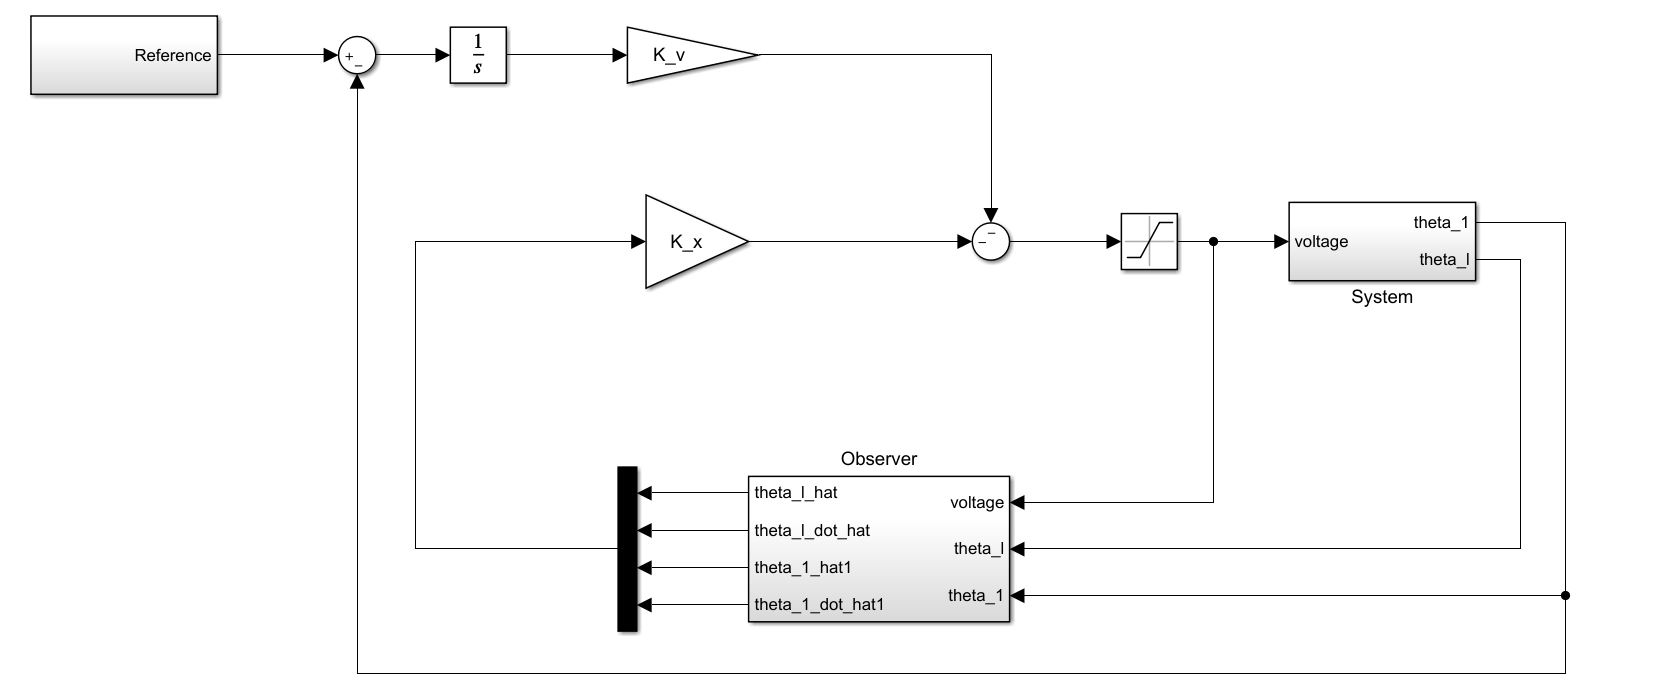
\includegraphics[scale=0.5]{pp_1}
	\caption{block scheme with pole placement and observer}
\end{figure*}

\newpage
At this point we set the poles through the \textit{place} matlab function. In particular we decide to postpone the real poles to speed up the system, whereas concerning the complex ones we just enhance their damping coefficients. At the beginning we thought to turn them into real poles but the resulting control effort was very aggressive and it was not leading any significant improvement to the dynamics.\\\\

\begin{equation}
	PlacedPoles^{T} =
	\begin{bmatrix}
		-20 \\ -50 \\ -40.1*(0.8+\sin(\arccos(0.8))*i) \\ -40.1*(0.8-\sin(\arccos(0.8))*i) \\-10  
	\end{bmatrix}
		K_x^{T} =
	\begin{bmatrix}
		185.9405 \\  3.5059 \\ -125.8645 \\   0.1222
	\end{bmatrix}
	\\
	K_v =
	\begin{bmatrix}
		286.2122
	\end{bmatrix}
\end{equation}

\begin{figure*}[h]
	\centering
	\begin{subfigure}{0.4\columnwidth}
		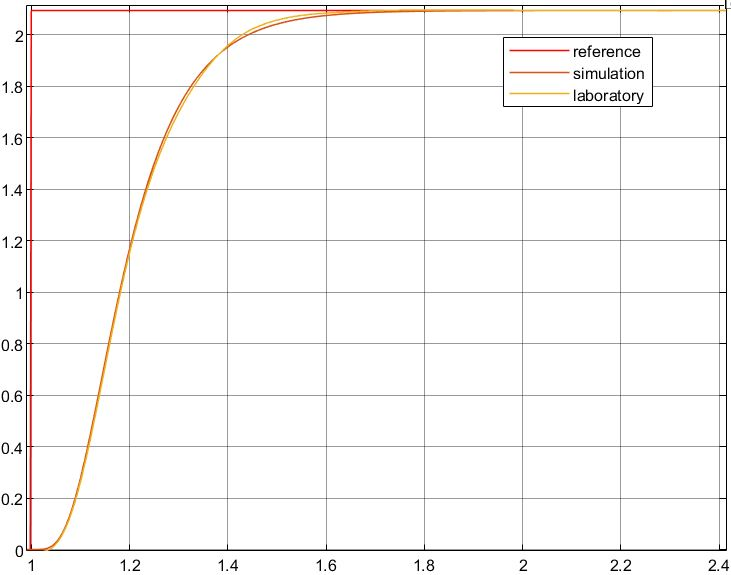
\includegraphics[width=\textwidth]{response_pp_1}
		\caption{Position}
	\end{subfigure}
	\begin{subfigure}{0.4\columnwidth}
		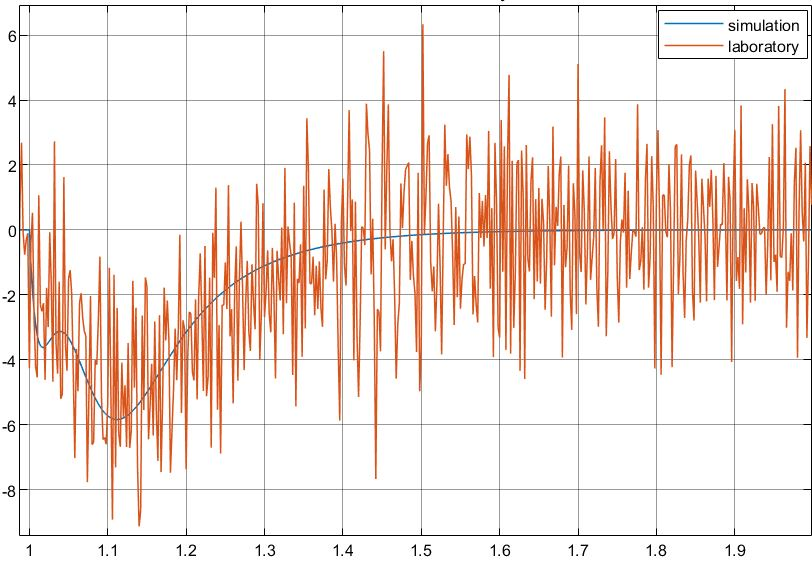
\includegraphics[scale=0.55]{voltage_pp_1}
		\caption{Voltage}
	\end{subfigure}
	\caption{position step response with dominant pole at 10 \textit{rad/s}}
\end{figure*}

We are already satisfied by this performance and we do not need to speed it up, however other solutions will be provided later on with LQG.

\section{2-DOF}
As before, we enlarge the system in order to reach the reference. The overall enlarged state space system is the following one:

\begin{equation}
	\begin{bmatrix}
		\dot{\theta_l} \\
		\ddot{\theta_l} \\
		\dot{\theta_1} \\
		\ddot{\theta_1} \\
		\dot{\theta_2} \\
		\ddot{\theta_2} \\
		\dot{v}
	\end{bmatrix}
	=
	\begin{bmatrix}
		0 &1 & 0 & 0 & 0 & 0 & 0 \\
		-\frac{K_{s_1}}{J_m} & -\frac{B_m}{J_m}-\frac{\eta_m \eta_g k_t k_m {K_g}^2}{R_m J_m}  & \frac{K_{s_1}}{J_m} & 0 & 0 & 0 & 0 \\
		0 & 0 & 0 & 1 & 0 & 0 & 0\\
		\frac{K_{s_1}}{J_1} & 0 & -\frac{K_{s_1}+K_{s_2}}{J_1} & -\frac{B_1}{J_1} & \frac{K_{s_2}}{J_1} & 0 & 0\\
		0 & 0 & 0 & 0 & 0 & 1 & 0 \\
		0 & 0 & \frac{K_{s_2}}{J_2} & 0 & -\frac{K_{s_2}}{J_2} & -\frac{B_2}{J_2} & 0 \\
		0 & 0 & 0 & 0 & 1 & 0 & 0
	\end{bmatrix}
	\begin{bmatrix}
		\theta_l \\
		\dot{\theta_l} \\
		\theta_1 \\
		\dot{\theta_1} \\
		\theta_2 \\
		\dot{\theta_2} \\
		v 
	\end{bmatrix}
	+
	\begin{bmatrix}
		0 \\
		\frac{\eta_m \eta_g k_t K_g}{R_m J_m} \\
		0 \\
		0 \\
		0 \\
		0 \\
		0 
	\end{bmatrix}
	V
 \end{equation}


\begin{figure*}[h]
	\centering
	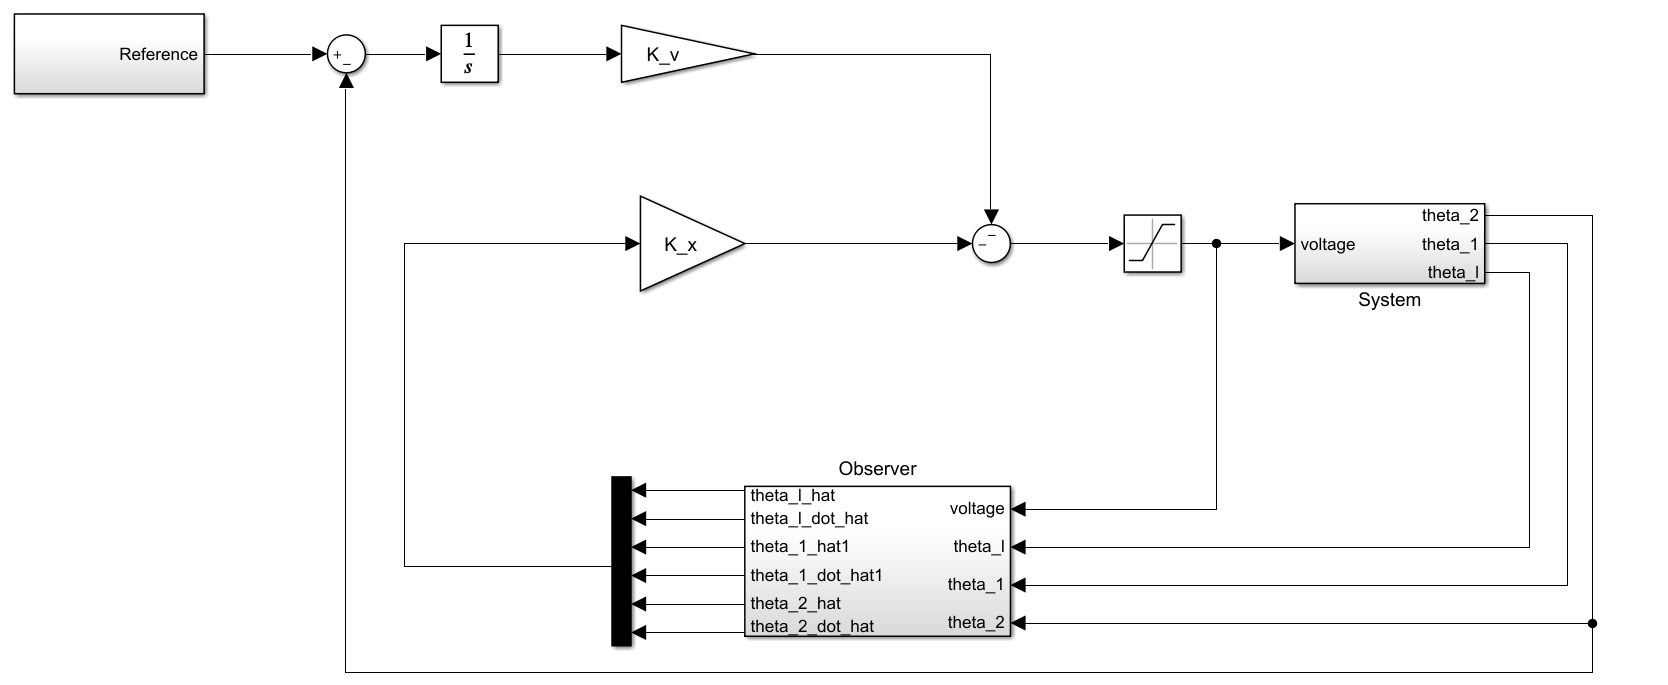
\includegraphics[scale=0.3]{pp_2}
	\caption{block scheme with pole placement and observer}
\end{figure*}

\newpage
Also in this case, we decide not to force the complex poles to real ones, but we just rise their damping coefficients. Below, it is possible to see where we placed the new poles of the system and the gain vector that lets us do it.

\begin{equation}
	PlacedPoles^{T} =
	\begin{bmatrix}
		-20 \\ -30 \\ -24.5*(0.6+\sin(\arccos(0.6))*i) \\ -24.5*(0.6-\sin(\arccos(0.6))*i) \\
		-61.9*(0.2+\sin(\arccos(0.2))*i) \\ -61.9*(0.2-\sin(\arccos(0.2))*i) \\ -10
	\end{bmatrix}
	K_x^{T} =
	\begin{bmatrix}
		68.1752  \\  1.1393 \\ -71.9542 \\   0.0150 \\  30.2715  \\  0.5489
	\end{bmatrix}
	\\
	K_v =
	\begin{bmatrix}
		110.9516
	\end{bmatrix}
\end{equation}

\begin{figure*}[h]
	\centering
	\begin{subfigure}{0.4\columnwidth}
		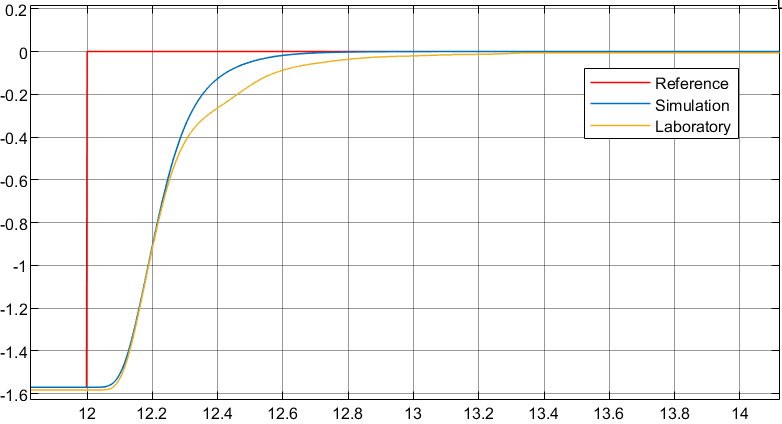
\includegraphics[width=\textwidth]{response_pp_2}
		\caption{Position}
	\end{subfigure}
	\begin{subfigure}{0.4\columnwidth}
		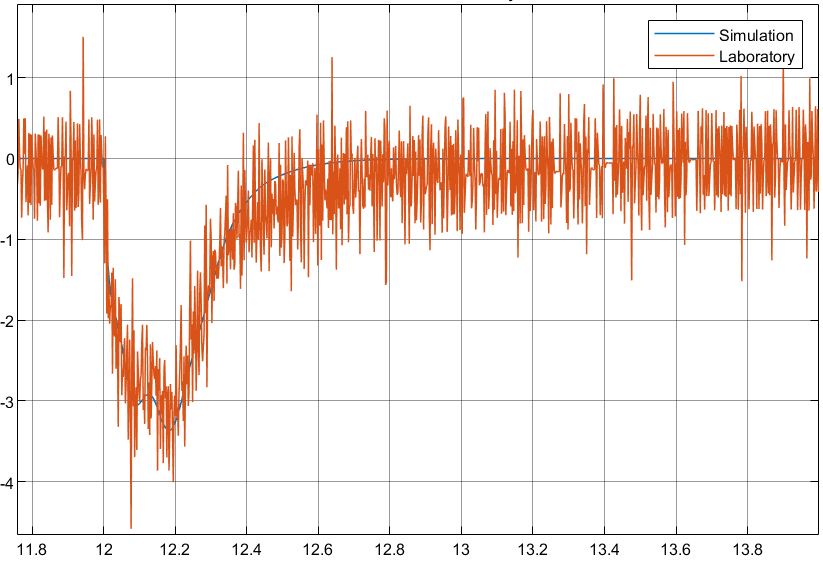
\includegraphics[scale=0.18]{voltage_pp_2}
		\caption{Voltage}
	\end{subfigure}
	\caption{position step response with dominant pole at 10 \textit{rad/s}}
\end{figure*}